% ============================================================
%  TASK 4.1 — TWO-DIODE RECTIFIER TOPOLOGY
% ============================================================

\section{Task 4.1 --- Two-Diode Rectifier Topology}
\label{sec:task4_1}

This part will present now the full characterization of the two-diode (voltage doubler) rectifier topology implemented with the HSMS-2862 Schottky diodes at an operating frequency of \SI{2.2}{\giga\hertz}. To increase the rectified output voltage and improve the overall power conversion efficiency, the single series diode is replaced by this new architecture. 

The analysis will follow the same systematic progression as in Task 3.1:
 (1) design and validation of the lumped-element (LC circuit) impedance matching circuit, and 
 (2) evaluation of the rectifier performance in terms of conversion efficiency~$\eta$, 
 output voltage~$V_\mathrm{out}$, and output current~$I_\mathrm{out}$ in Task 4.2.

% ------------------------------------------------------------
\subsection{Two-Diode Input Impedance Characterization}
\label{subsec:2d_zin}
% ------------------------------------------------------------

Before designing the matching network, the input impedance $Z_\mathrm{in}$ of the two-diode voltage doubler must be extracted. Just like in the one-diode topology, an LSSP simulation is performed at \SI{2.2}{\giga\hertz}, but this time with a fixed load of $R_L = \SI{20}{\kilo\ohm}$ to match the sensor requirements.
Here is the schematic done for this : 

\begin{figure}[H]
    \centering
    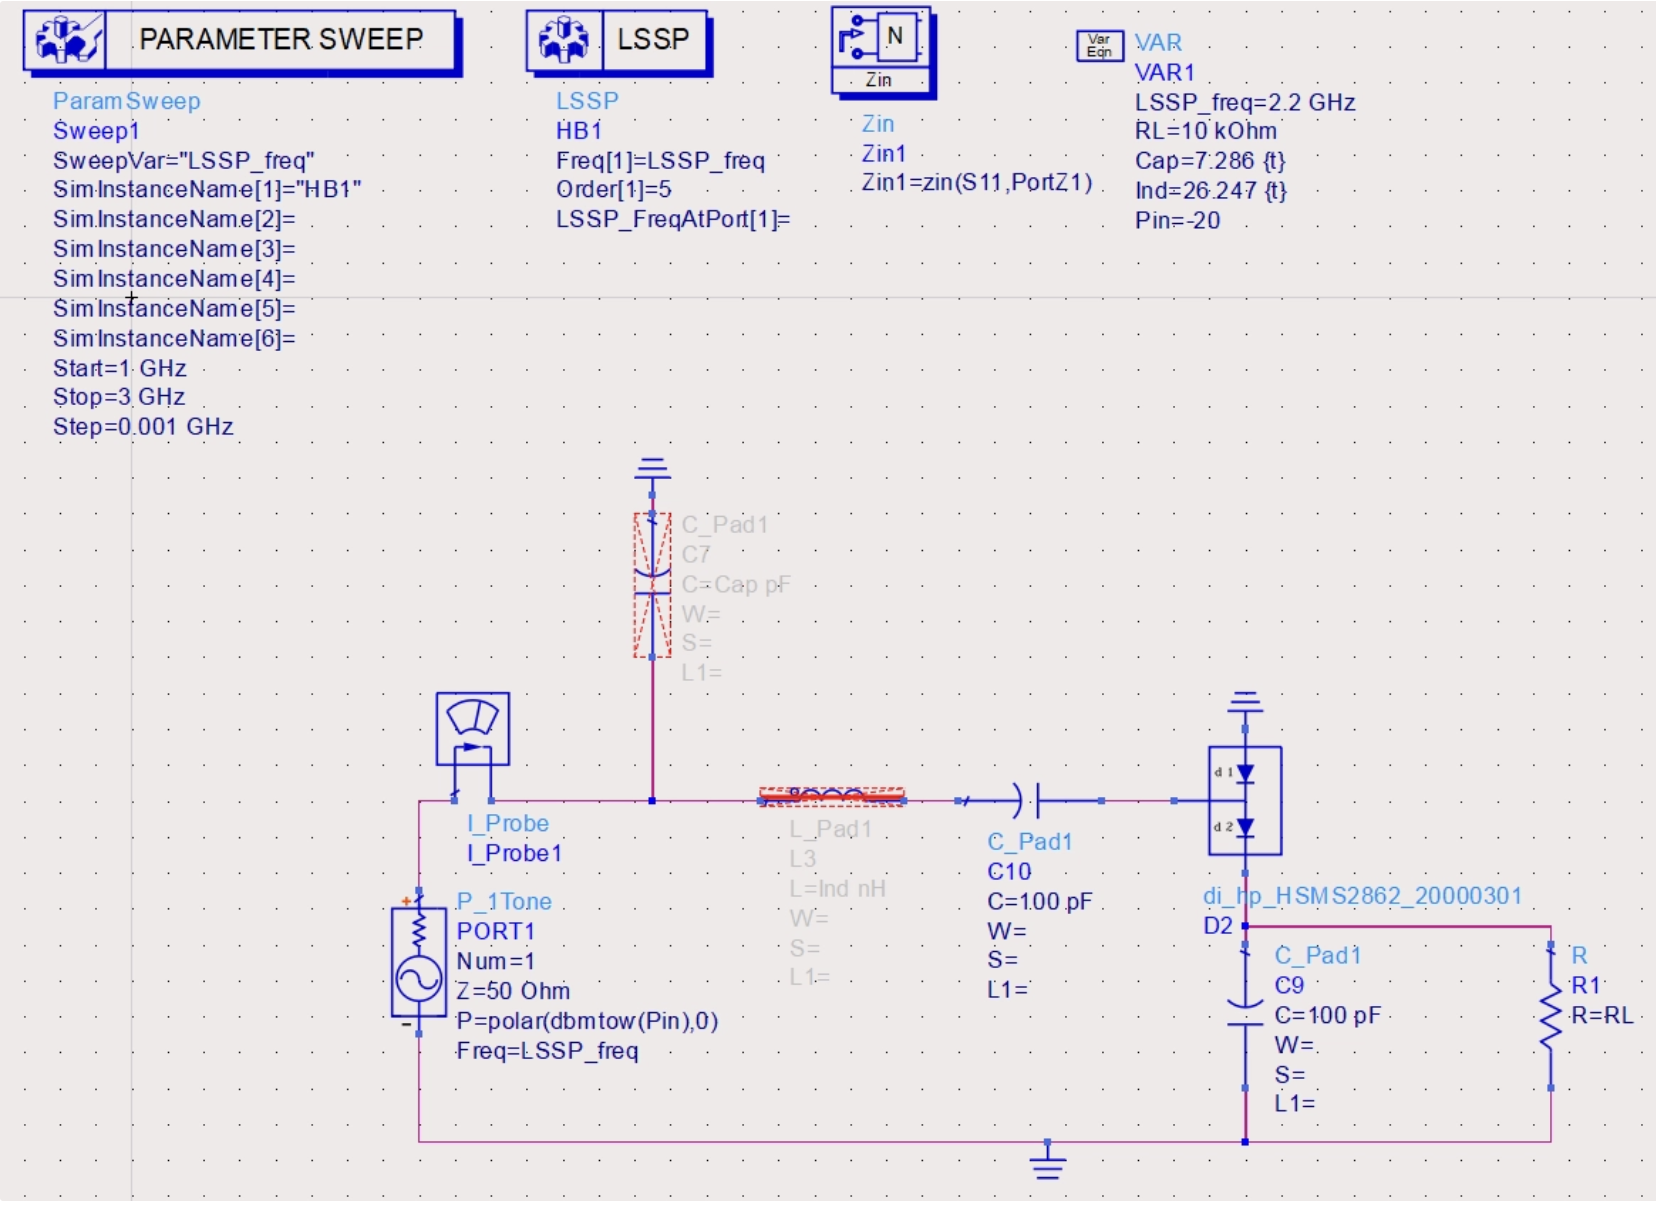
\includegraphics[width=\linewidth]{images/sch_2d.png} 
    \caption{2 diodes circuit to determine $Z_\mathrm{in}$ of the two-diode}
    \label{fig:sch_2d_LC}
\end{figure}

Table~\ref{tab:zin_vs_pin_2d} summarizes the extracted impedance values for different input power levels.

\begin{table}[H]
    \centering
    \caption{Real and imaginary parts of $Z_\mathrm{in}$ for the two-diode topology at \SI{2.2}{\giga\hertz} depending on $P_\mathrm{in}$, with $R_L = \SI{20}{\kilo\ohm}$.}
    \label{tab:zin_vs_pin_2d}
    \begin{tabular}{S[table-format=-2.0]
                    S[table-format=1.3]
                    S[table-format=-3.3]}
        \toprule
        {$P_\mathrm{in}$ (dBm)} &
        {$\mathrm{Re}(Z_\mathrm{in})$ ($\Omega$)} &
        {$\mathrm{Im}(Z_\mathrm{in})$ ($\Omega$)} \\
        \midrule
        -30 & 3.238 & -123.639 \\
        -20 & 3.111 & -125.109 \\
        -10 & 2.923 & -131.755 \\
          0 & 2.766 & -149.336 \\
         10 & 3.393 & -188.751 \\
        \bottomrule
    \end{tabular}
\end{table}

Compared to the single-diode topology, the real part is low and stable (around \SI{3}{\ohm}), but the imaginary part is very less negative (around \SI{-125}{\ohm} at \SI{-20}{\dBm}, compared to \SI{-263}{\ohm} for the single diode). This massive variation confirms that the previous matching network cannot be reused and a completely new one must be designed.

% ------------------------------------------------------------
\subsection{Lumped Element Impedance Matching Circuit}
\label{subsec:2d_matching_lumped}
% ------------------------------------------------------------

\subsubsection{Design methodology}

The two-diode rectifier consists of a shunt diode and a series diode. During the negative half-cycle of the input RF signal, the shunt diode conducts and charges the series input capacitor. During the positive half-cycle, the series diode conducts, transferring the charge to the output capacitor, effectively doubling the peak voltage.

Because of this new architecture, the objective of the matching circuit is to transform the antenna source impedance $Z_0 = \SI{50}{\ohm}$ to the complex conjugate of the newly extracted input impedance (Table~\ref{tab:zin_vs_pin_2d}) to maximize power transfer. 

The design employs the same ADS dynamic tuning tool (\emph{Tune}) with ideal SMD components. The target specification at \SI{2.2}{\giga\hertz} remains $S_{11} < \SI{-10}{\deci\bel}$, with the load resistance fixed at $R_L = \SI{20}{\kilo\ohm}$.

\begin{figure}[H]
    \centering
    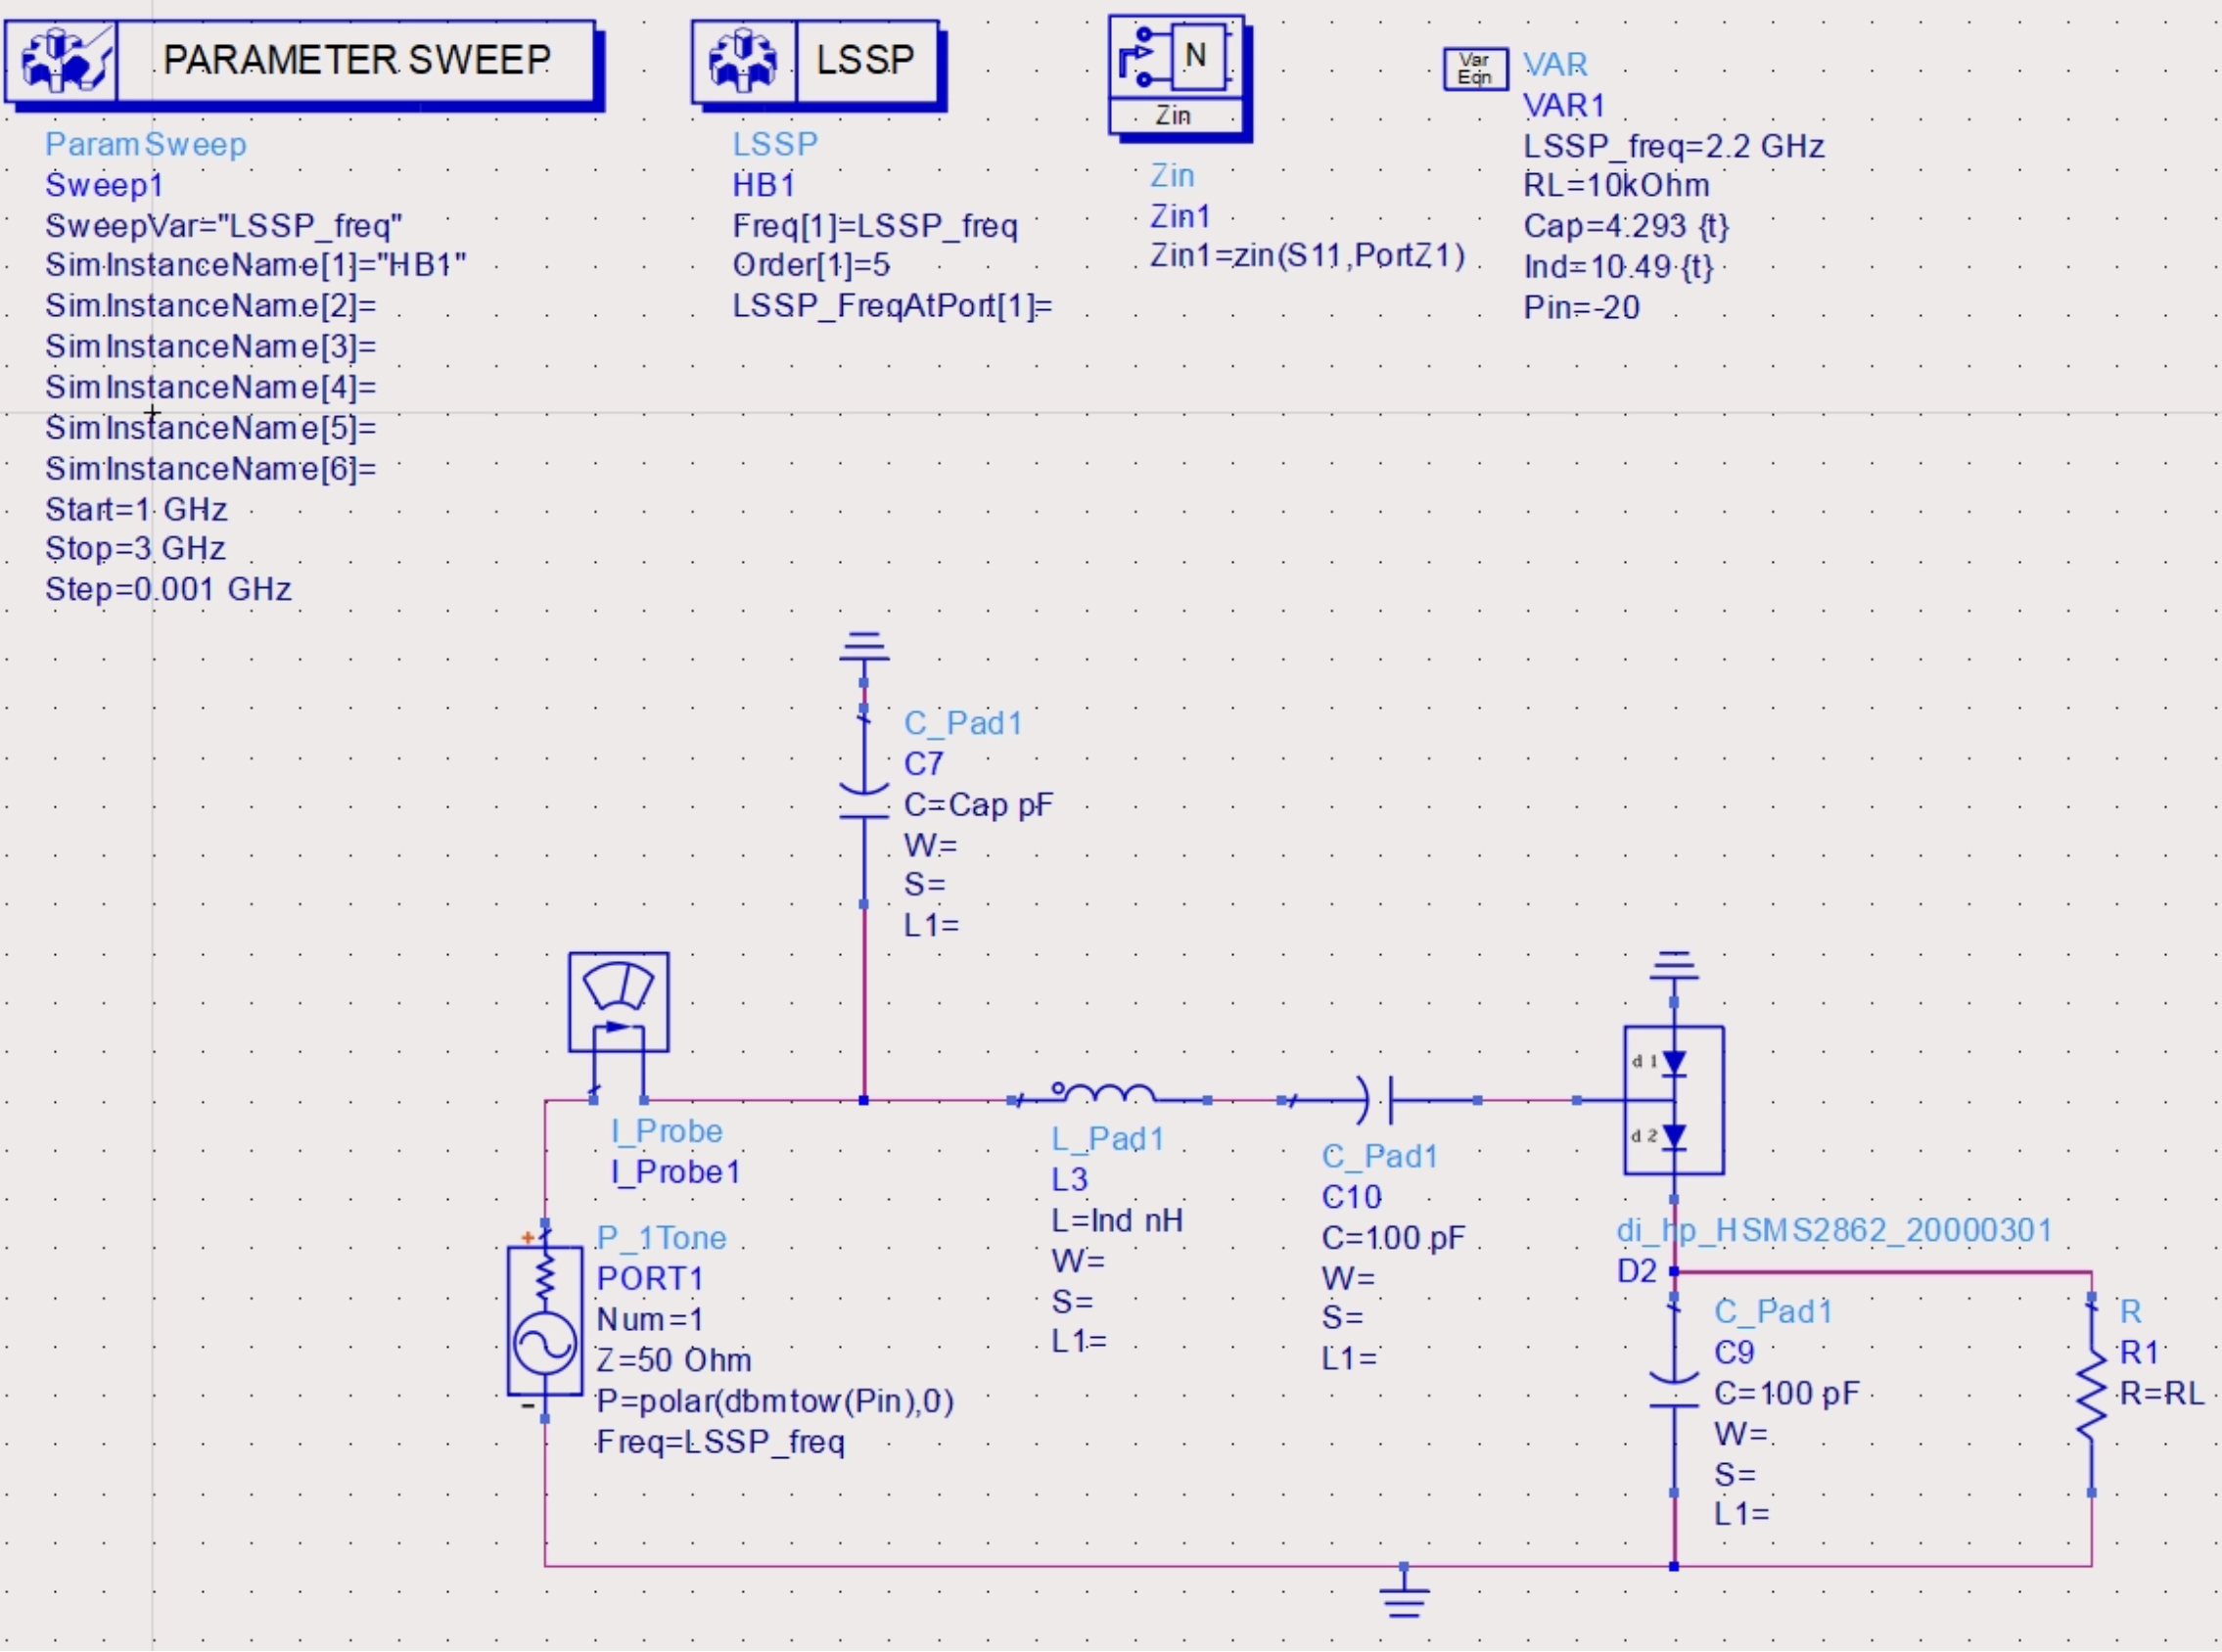
\includegraphics[width=\linewidth]{images/schema_2d_lc.png} % <-- Schéma ADS 2 diodes en composants LC idéaux
    \caption{ADS schematic of the two-diode voltage doubler rectifier and LC matching circuit.}
    \label{fig:schema_2d_lc_matching}
\end{figure}

\subsubsection{Results after tuning}

After optimization, the tuning successfully centers the resonance at \SI{2.2}{\giga\hertz}. 

\begin{figure}[H]
    \centering
    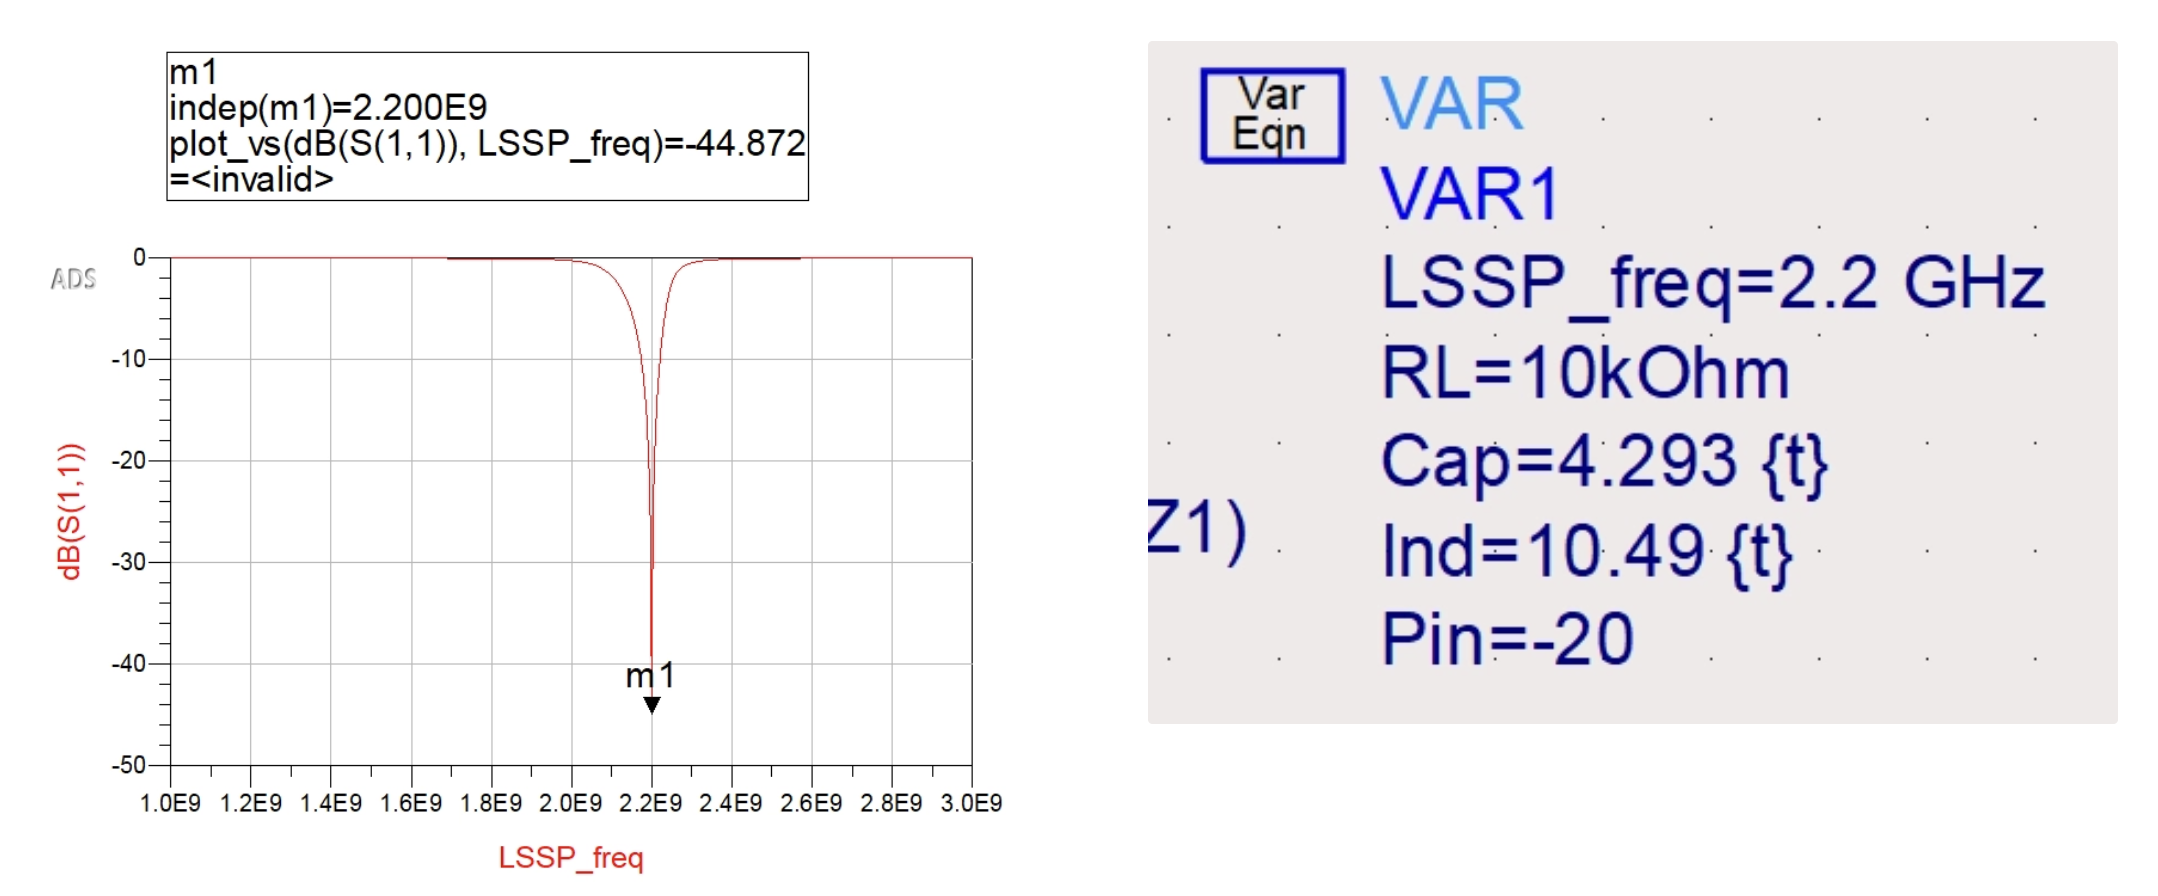
\includegraphics[width=0.75\linewidth]{images/s11_2d_lc.png} % <-- Graphique du S11 avec composants LC
    \caption{$S_{11}$ parameter of the two-diode rectifier with the LC matching circuit.}
    \label{fig:s11_2d_lc}
\end{figure}

The condition $S_{11} < \SI{-10}{\deci\bel}$ is met with the optimized component values of $C = \SI{4.293}{\pico\farad}$ and $L = \SI{10.49}{\nano\henry}$, confirming a good impedance match before introducing the microstrip lines.